\begin{tikzpicture}
%*** First graph ***
\draw[->, thick] (-2,0)  --  (2,0) node[right] {$x$};
\draw[->, thick] (0,-.3)  --  (0,1.5) node[right] {$y$};
\draw[very thick, blue] (-2,0)--(-0.4,0);
\draw[very thick, blue] (-0.4,0.8)--(2,0.8) node[right] {$F_{X_n}$};
\draw[thin, dashed] (-0.4,0)--(-0.4,0.8);
	\draw[very thick] (-0.4,-0.2) node[below]{$-\tfrac{1}{n}$} -- (-0.4,0);
\filldraw[color=blue, fill=white,  very thick](-0.4,0) circle (0.05);
\filldraw[color=blue, fill=blue,  very thick](-0.4,0.8) circle (0.05);

%*** Second graph ***
\begin{scope}[xshift=6cm]
\draw[->, thick] (-2,0)  --  (2,0) node[right] {$x$};
\draw[->, thick] (0,-.3)  --  (0,1.5) node[right] {$y$};
\draw[very thick, red] (-2,0)--(0.4,0);
\draw[very thick, red] (0.4,0.8)--(2,0.8) node[right] {$F_{Y_n}$};
\draw[thin, dashed] (0.4,0)--(0.4,0.8);
	\draw[very thick] (0.4,-0.2) node[below]{$\tfrac{1}{n}$} -- (0.4,0);
\filldraw[color=red, fill=white,  very thick](0.4,0) circle (0.05);
\filldraw[color=red, fill=red,  very thick](0.4,0.8) circle (0.05);
\end{scope}

%*** Third graph ***
\begin{scope}[xshift=12cm]
\draw[->, thick] (-2,0)  --  (2,0) node[right] {$x$};
\draw[->, thick] (0,-.3)  --  (0,1.5) node[right] {$y$};
\draw[very thick, purple] (-2,0)--(0,0);
\draw[very thick, purple] (0,0.8)--(2,0.8) node[right] {$F_{Z}$};
\draw[thin, dashed] (0,0)--(0,0.8);
\filldraw[color=purple, fill=white,  very thick](0,0) circle (0.05);
\filldraw[color=purple, fill=purple,  very thick](0,0.8) circle (0.05);
\end{scope}

\end{tikzpicture}

